\documentclass[12pt, a4paper]{article}
\usepackage[utf8]{inputenc}
\usepackage[margin=1in]{geometry}
\usepackage[toc, page]{appendix}
\usepackage{multirow}
\usepackage{pdflscape}
\usepackage{array}
\usepackage{longtable}
\usepackage{color} 
\usepackage[pdftex]{hyperref}
\hypersetup{
	colorlinks=true,
	linktoc=all,
	linkcolor=black,
}
\usepackage[export]{adjustbox}
\usepackage{float}
\restylefloat{table}
\usepackage{array}
\usepackage[activate={true,nocompatibility},final,tracking=true,kerning=true,spacing=true,factor=1100,stretch=10,shrink=10]{microtype}
\usepackage{tikz}
\usepackage{graphicx}
\usepackage{pgfplots}
\usepackage{multirow}
\usepackage{callouts}
\usepackage{longtable}
\usepackage{array}
\usepackage[justification=centering]{caption} 
\usetikzlibrary{intersections}
\usepackage{fontawesome}
\usepackage{capt-of}

\newlength\colB \setlength\colB{5cm}
\newlength\colC \setlength\colC{5cm}
\newlength\combinedlength 
\setlength\combinedlength{%
	\dimexpr\colB+\colC+4\tabcolsep+%
	2\arrayrulewidth\relax}

\title{MYP Economics G2 01 - Taxation}
\author{Adithya Narayanan}
\date{20 September, 2019}

\begin{document}
	\begin{titlepage}
		\maketitle
		\begin{center}
			Word count: 1500
		\end{center}
	\end{titlepage}
	\tableofcontents
	\newpage
	\section{Introduction}
	Tax systems play a crucial role in economies and can be manipulated by governments for the purpose of achieving macroeconomic aims. Tax systems determine the budget of a government and remains the main source of revenue for governments around the world. However, different tax systems can engender different effects on an economy.
	\section{Fiscal policy}
	The Fiscal policy is a defined as "Manipulations by the government of its own expenditures and taxes in order to influence the level of aggregate demand; it is a type of demand- side policy or demand management"(Tragakes 544). This is achieved by influencing the components of AD thus curbing or stimulating the economy.
	\newline
	
	In expansionary fiscal policies, government spending may be increased, while taxes(T) may be decreased(See Fig.1). These shift the AD curve to the right(See Fig.2), allowing the economy to approach full employment of resources. The end result is an increase in Real GDP from $ Y_{rec} $ to $ Y_{p} $, hence used where a government needs to stimulate an economy(during recessions).
	
	\begin{figure}[H]
		\begin{center}
			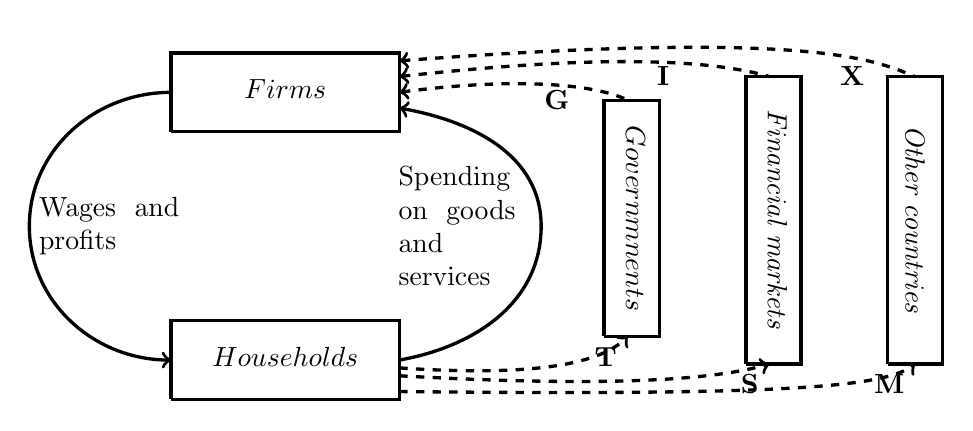
\begin{tikzpicture}[scale=1.0]
			\draw[very thick] (1.8, 0) -- (4.7, 0) -- (4.7, 1) -- (1.8, 1) -- (1.8, 0);
			\draw[very thick] (1.8, 3.4) -- (4.7, 3.4) -- (4.7, 4.4) -- (1.8, 4.4) -- (1.8, 3.4);
			\draw[very thick] (7.3, 0.8) -- (8, 0.8) -- (8, 3.8) -- (7.3, 3.8) -- (7.3, 0.8);
			\draw[very thick] (9.1, 0.45) -- (9.8, 0.45) -- (9.8, 4.1) -- (9.1, 4.1) -- (9.1, 0.45);
			\draw[very thick] (10.9, 0.45) -- (11.6, 0.45) -- (11.6, 4.1) -- (10.9, 4.1) -- (10.9, 0.45);
			
			\draw [very thick, ->] (1.8, 3.9) to [out=-180, in=90] (0, 2.2) to [out=-90, in=180] (1.8, 0.5);
			\draw [very thick, ->] (4.7, 0.5) to [out=10, in=-90] (6.5, 2.2) to [out=90, in=-10] (4.7, 3.7); 
			
			\draw [very thick, ->] [dashed] (4.7, 0.4) ..controls (6.2, 0.3) and (7.2, 0.4) ..(7.6, 0.8) node [below left] {$\textbf{T}$}; 
			\draw [very thick, ->] [dashed] (4.7, 0.3) ..controls (7.4, 0.15) and (8.7, 0.25) ..(9.4, 0.45) node [below left] {$\textbf{S}$};
			\draw [very thick, ->] [dashed] (4.7, 0.1) ..controls (9.55, 0.05) and (10.85, 0.15) ..(11.25, 0.45) node [below left] {$\textbf{M}$};			
			
			\draw [very thick, <-] [dashed] (4.7, 3.9) ..controls (6.2, 4.1) and (7.2, 4) ..(7.6, 3.8); 
			\draw [very thick, <-] [dashed] (4.7, 4.1) ..controls (7.4, 4.4) and (8.7, 4.3) ..(9.4, 4.1);
			\draw [very thick, <-] [dashed] (4.7, 4.3) ..controls (10, 4.7) and (10.75, 4.3) ..(11.25, 4.1);
			
			\node [above] at (3.25, 0.3) {$Households$}; 
			\node [above] at (3.25, 3.7) {$Firms$};
			\node [below] at (6.7, 4.05) {$\textbf{G}$}; 
			\node [below] at (8.05, 4.35) {$\textbf{I}$}; 
			\node [below] at (10.45, 4.35) {$\textbf{X}$}; 
			\node at (7.7, 2.3){\rotatebox{-90}{$Governmnents$}}; 
			\node at (9.5, 2.275){ \rotatebox{-90}{\textit{Financial markets}}}; 
			\node at (11.25, 2.275){ \rotatebox{-90}{\textit{Other countries}}}; 
			
			\node at (0, 2.2) [align = left, right] {Wages \ and \\ profits}; 
			
			\node at (6.3, 2.2) [align = left, left] {Spending \\ on \ goods \\ and \\ services};
			\end{tikzpicture}
		\end{center}
		\caption{Narayanan, Adithya. \textit{Circular Flow of Income, G Increases and T Decreases}.}
		
		Contractionary policies have the inverse effect on an economy. When an economy experiences an inflationary gap, governments may increase taxes and decrease expenditures, to shift the AD curve to the left and is used to achieve the aim of maintaining low inflation.
		
	\end{figure}
	\begin{figure}[H]
		\caption{Narayanan, Adithya. \textit{Aggregate demand and supply diagram during the implementation of an expansionary fiscal policy}.}
		\begin{center}
			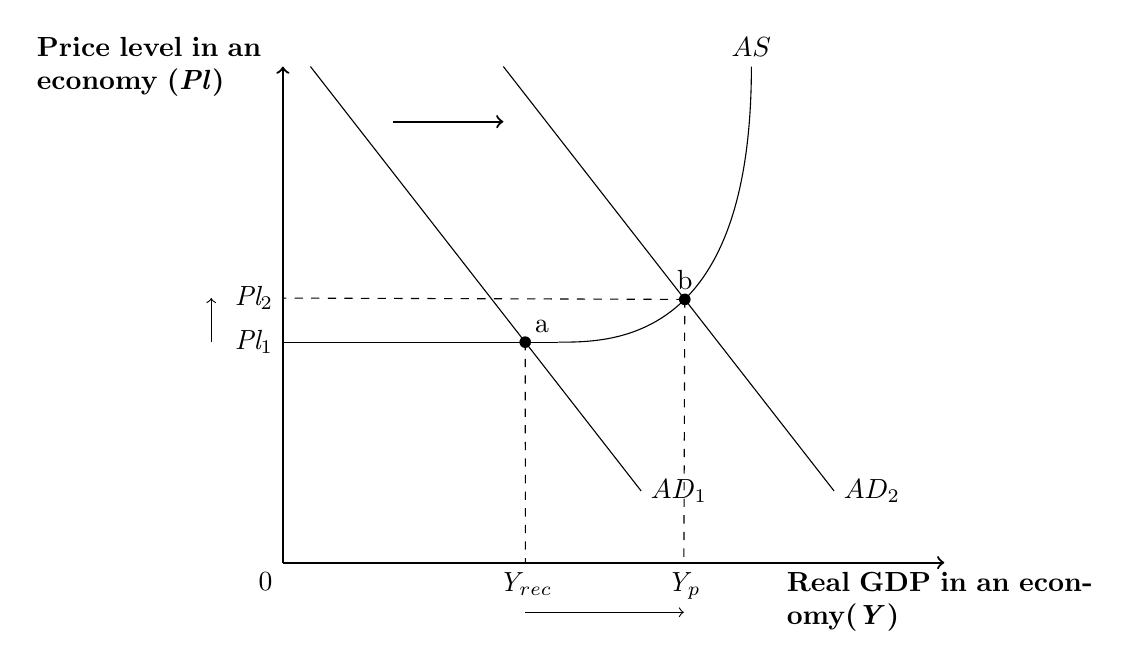
\begin{tikzpicture}[scale = 0.7]
			\draw[thick, <-] (0,9) -- (0,0) node[below left]{$0$};
			\draw[thick, ->] (0,0) -- (12,0);
			\node[below, text width = 4 cm] at (12, 0) {\textbf{Real GDP in an economy(\textit{Y})}}; 
			\node[left, text width = 3 cm] at (0,9) {\textbf{Price level in an economy (\textit{Pl})}};
			
			\draw[name path = AD1] (6.5,1.3) node[right]{$AD_{1}$} -- (0.5, 9);
			\draw[name path = AD2] (10,1.3) node[right]{$AD_{2}$} -- (4, 9);
			\draw[->, thick] (2.0, 8) -- (4, 8);
			\draw[name path = ASflat] (0, 4) node[left]{\textit{Pl$  _{1} $}} -- (5,4);
			\draw[name path= AS] (5, 4) ..controls (6, 4) and (8.5, 4) .. (8.5, 9) node[above]{$ AS $};
			\fill [black, name intersections={of=AD1 and ASflat}] (intersection-1)circle (3pt) node[above right]{a};
			\draw[dashed] (intersection-1) -- (4.4,0) node[below]{\textit{Y$ _{rec} $}};
			\fill [black, name intersections={of=AD2 and AS}] (intersection-1)circle (3pt) node[above]{b};
			\draw[dashed] (intersection-1) -- (7.275,0) node[below]{\textit{Y$ _{p} $}};
			\draw[dashed] (intersection-1) -- (0,4.8) node[left]{\textit{Pl$ _{2} $}};
			\draw[->] (-1.3,4) -- (-1.3, 4.8);
			\draw[->] (4.4, -0.9) -- (7.275, -0.9);
			\end{tikzpicture}
		\end{center}
	\end{figure}
	
	\section{Tax systems:}
	\subsection{Progressive:}
	The term progressive tax system is used to indicate that "high-income earners [are taxed] proportionately more than low-income earners"(Poh). As income increases, the proportion taken in tax also rises. "The rationale is that people with a lower income will usually spend a greater percentage of their income to maintain their standard of living."(Investopedia).
	\newline
	
	The term progressive may also be used to describe the degree by which the proportion of income taken as tax increases as income increases, hence used to compare relative differences between progressive systems.
	
	\subsection{Regressive:}
	In regressive tax systems, those with lower incomes are taxed proportionately more than those with higher incomes, the inverse of progressive tax systems. As income increases, the proportion taxed decreases.
	
	\subsection{Proportional direct:}
	In Proportional direct or flat tax systems, the proportion of income taken as tax is unchanged, regardless of income.
	\newpage
	\section{Singapore}
	\subsection{Income tax:}
	Income tax in Singapore for tax residents in each financial year(FA) is progressive(See Fig.3). Tax residents are individuals who have stayed or worked in Singapore for a minimum 183 days in a year, or "for a period straddling two calendar years and ... total period of stay is at least 183 days"(Inland Revenue authority of Singapore). Individuals who are public entertainers, professionals or directors of a company as these individuals are classified as non-tax residents regardless. Taxable income sources include income earned in Singapore and "foreign-sourced income that was brought into Singapore prior to 1 Jan 2004"(Inland Revenue authority of Singapore); income brought into Singapore following 1 Jan 2004 is exempt from taxation.
	\newline
	
	Non-tax residents are charged a flat 15\% (See Fig.4) or progressive tax, depending on which method of taxation results in higher tax paid, which is calculated to be an income above S\$369,286. Disposable income is calculated using:
	
	\begin{equation}
	Disposable \ yearly \ income = Yearly \ income - Gross \ payable \ tax
	\end{equation}
		
		\vspace{-2em}
		\begin{figure}[H]
			\begin{longtable}{|>{\centering\arraybackslash}m{2.4cm}|>{\centering\arraybackslash}m{4.9cm}|>{\centering\arraybackslash}m{3.2cm}|>{\centering\arraybackslash}m{4cm}|}
				\cline{2-4}
				\multicolumn{1}{c|}{} & \textbf{Chargeable yearly income bracket (S\$)} & \textbf{Income tax rate (\%)} & \textbf{Gross payable tax (S\$)}\\
				\cline{2-4}
				\hline
				\underline{On the first} & 20,000 & 0.0 & 0\\
				\hline
				\textit{On the next} & 10,000 & 2.0 & 200\\
				\hline
				\underline{On the first} & 30,000 & - & 200\\
				\hline
				\textit{On the next} & 10,000 & 3.5 & 350\\
				\hline
				\underline{On the first} & 40,000 & - & 550\\
				\hline
				\textit{On the next} & 40,000 & 7.0 & 2,800\\
				\hline
				\underline{On the first} & 80,000 & - & 3,350\\
				\hline
				\textit{On the next} & 40,000 & 11.5 & 4,600\\
				\hline
				\underline{On the first} & 120,000 & - & 7,950\\
				\hline
				\textit{On the next} & 40,000 & 15.0 & 6,000\\
				\hline
				\underline{On the first} & 160,000 & - & 13,950\\
				\hline
				\textit{On the next} & 40,000 & 18.0 & 7,200\\
				\hline
				\underline{On the first} & 200,000 & - & 21,150\\
				\hline
				\textit{On the next} & 40,000 & 19.0 & 7,600\\
				\hline
				\underline{On the first} & 240,000 & - & 28,750\\
				\hline
				\textit{On the next} & 40,000 & 19.5 & 7,800\\
				\hline
				\underline{On the first} & 280,000 & - & 36,550\\
				\hline
				\textit{On the next} & 40,000 & 20 & 8000\\
				\hline
				\underline{On the first} & 320,000 & - & 44,550\\
				\hline
				\textit{Above} & 320,000 & 22 & -\\
				\hline
			\end{longtable}
			\caption{ Inland Revenue Authority of Singapore. \textit{Resident Tax Rates From YA 2017 Onwards}.Table.}
		\end{figure}

		\begin{figure}[H]
			\begin{longtable}{|>{\centering\arraybackslash}m{2.4cm}|>{\centering\arraybackslash}m{4.9cm}|>{\centering\arraybackslash}m{3.2cm}|>{\centering\arraybackslash}m{4cm}|}
				\cline{2-4}
				\multicolumn{1}{c|}{} & \textbf{Chargeable yearly income bracket (S\$)} & \textbf{Income tax rate (\%)} & \textbf{Gross payable tax (S\$)}\\
				\cline{2-4}
				\cline{1-2}\cline{4-4}
				\underline{On the first} & 20,000 & \multirow{23}{3.2cm}{\centering 15.0} & 3,000\\
				\cline{1-2}\cline{4-4}
				\textit{On the next} & 10,000 &  & 1,500\\
				\cline{1-2}\cline{4-4}
				\underline{On the first} & 30,000 &  & 4,500\\
				\cline{1-2}\cline{4-4}
				\textit{On the next} & 10,000 &  & 1,500\\
				\cline{1-2}\cline{4-4}
				\underline{On the first} & 40,000 &  & 6,000\\
				\cline{1-2}\cline{4-4}
				\textit{On the next} & 40,000 & & 6,000\\
				\cline{1-2}\cline{4-4}
				\underline{On the first} & 80,000 & & 12,000\\
				\cline{1-2}\cline{4-4}
				\textit{On the next} & 40,000 &  & 6,000\\
				\cline{1-2}\cline{4-4}
				\underline{On the first} & 120,000 &  & 18,000\\
				\cline{1-2}\cline{4-4}
				\textit{On the next} & 40,000 &  & 6,000\\
				\cline{1-2}\cline{4-4}
				\underline{On the first} & 160,000 &  & 24,000\\
				\cline{1-2}\cline{4-4}
				\textit{On the next} & 40,000 &  & 6,000\\
				\cline{1-2}\cline{4-4}
				\underline{On the first} & 200,000 &  & 30,000\\
				\cline{1-2}\cline{4-4}
				\textit{On the next} & 40,000 &  & 6,000\\
				\cline{1-2}\cline{4-4}
				\underline{On the first} & 240,000 &  & 36,000\\
				\cline{1-2}\cline{4-4}
				\textit{On the next} & 40,000 &  & 6,000\\
				\cline{1-2}\cline{4-4}
				\underline{On the first} & 280,000 &  & 42,000\\
				\cline{1-2}\cline{4-4}
				\textit{On the next} & 40,000 &  & 6,000\\
				\cline{1-2}\cline{4-4}
				\underline{On the first} & 320,000 &  & 48,000\\
				\cline{1-2}\cline{4-4}
				\textit{On the next} & 40,000 &  & 6,000\\
				\cline{1-2}\cline{4-4}
				\underline{On the first} & 360,000 &  & 54,000\\
				\cline{1-2}\cline{4-4}
				\textit{On the next} & 9,285 &  & 1392.75\\
				\cline{1-2}\cline{4-4}
				\underline{On the first} & 369,285 &  & 55,392.75\\
				\hline
				\textit{Above} & 369,286 &  Refer to progressive tax resident system & Refer to progressive tax resident system \\
				\hline
			\end{longtable}
			\caption{Inland Revenue Authority of Singapore. \textit{Tax Rates for Non-Residents}. Table.}
		\end{figure}

		\subsection{Direct taxes:}
		\subsubsection{Corporate tax:}
		Singapore imposes flat corporate taxes on tax resident firms' profits up till S\$300,000 of 8.5\%. Profits above S\$300,000 are charged 17\%. No tax is charged on capital gains, dividend distribution amongst shareholders and foreign sourced income not brought into Singapore for corporations.
		\newline
		
		Firms do not have to incur double payments in 76 countries that have signed "Avoidance of Double taxation Agreements(DTAs)"(Inland revenue authority of Singapore).
		
		
		\subsection{Indirect taxes:}
		\subsubsection{Government service tax:}
		A flat 7\% is charged on all goods and services sold in Singapore(Ministry of Finance). Although this is a flat rate, it can also be considered regressive, as individuals with lower incomes would be spending a higher proportion of their income, than those with higher incomes. Real estate sales, supply and investment of precious metals, financial services, exports of goods and international services, and financial services are all exempt from GST and are zero rated.
		
		\subsubsection{Excise duties:}
		Goods and services are taxed under 4 different categories, with varying subcategories. Taxes for each unit of a good that falls in one of the above categories is calculated using specific formulas(See Fig.5). Excise duty rates(EDRs) refer to over 509 percentage values set by the government for different types of goods.
				\begin{figure}[H]
					\centering
					\begin{tabular}{|>{\centering\arraybackslash}m{3.17cm}|>{\centering\arraybackslash}m{5.17cm}|>{\centering\arraybackslash}m{5.27cm}|}
						\cline{2-3}
						\multicolumn{1}{c|}{}& \textbf{Product:} & \textbf{Formula:}\\
						\hline
						\multirow{2}{3.17cm}{\centering Intoxicating liquor} & Alcoholic products with EDR based on per litre of alcohol & Quantity(L)$\times$EDR$\times$Alcoholic strength(\%)\\
						\cline{2-3}
						& Alcoholic products with EDR based on volume or weight & Dutiable quantity(kg)$\times$EDR\\
						\hline
						\multirow{2}{3.17cm}{\centering Tobacco} & Tobacco products excluding cigarettes & Weight(kg)$\times$EDR\\
						\cline{2-3}
						& Cigarettes & Number of cigarettes(individual)$\times$Weight of each cigarette(g)$\times$EDR\\
						\hline
						Motor vehicles & Motor vehicles & Customs value$\times$EDR\\
						\hline
						\multirow{3}{3.17cm}{\centering Petroleum and biodiesel} & Compressed natural gas & Weight$\times$EDR\\
						\cline{2-3}
						& Biodiesel blends & Volume$\times$EDR\\
						\cline{2-3}
						& Compressed natural gas & Weight$\times$EDR\\
						\hline
					\end{tabular}
					\caption{Singapore customs. \textit{Duties and Dutiable Goods}. Table.}
				\end{figure}
		
			\subsubsection{Motor vehicles tax/licenses:}
				There are 3 main taxes imposed on vehicles in Singapore - Road tax(See Fig.4), diesel tax and surcharge on tax(See Fig.5). Road tax in Singapore is based on engine capacity(EC).
				
				\begin{figure}[H]
					\begin{tabular}{|>{\centering\arraybackslash}m{7.76cm}|>{\centering\arraybackslash}m{7.76cm}|}
						\hline
						\textbf{EC(cc)} & \textbf{Formula, per YA}\\
						\hline
						\hline
						\textit{Less than} 600 & S\$400$\times$0.72\\
						\hline
						600-1000 & [S\$400+0.25$\times$(EC - 600)]$\times$0.782\\
						\hline
						1001-1600 & [S\$500+0.75$\times$(EC - 1000)]$\times$0.782\\
						\hline
						1601-3000 & [S\$950+1.5$\times$(EC - 1600)]$\times$0.782\\
						\hline
						\textit{Greater than} 3000 & [S\$3050+2.0$\times$(EC - 3000)]$\times$0.782\\
						\hline
					\end{tabular}
				\caption{SGCarMart.com. \textit{Road Tax Formulas}. Table.}
				\end{figure}	
				
				Tax on diesel vehicles who fall below emission standards of Euro 4, are taxed S\$1.25 per cc. Vehicles with emission standards above Euro 5 are taxed S\$0.40 per cc.
				\newline

				Road tax surcharges are added based on the age of the vehicle and calculated with:
		
				\begin{equation}
					Total \ tax = Road \ tax \times(1+surcharge)
				\end{equation}
				
				\begin{figure}[H]
					\begin{tabular}{|>{\centering\arraybackslash}m{7.76cm}|>{\centering\arraybackslash}m{7.76cm}|}
						\hline
						\textbf{Vehicle age(Above no. of years)} & \textbf{Road tax surcharge, per YA(\%)}\\
						\hline
						\hline
						10 & 10\\
						\hline
						11 & 20\\
						\hline
						12 & 30\\
						\hline
						13 & 40\\
						\hline
						14 & 50\\
						\hline
					\end{tabular}
					\caption{SGCarMart.com. \textit{Road Tax Surcharge (For Vehicle over 10 Years)}.Table.}
				\end{figure}	
				\newpage

\section{Russia:}
\subsection{Income tax:}
Income tax in Russia is a flat 13\% for tax residents(See Fig.3) and 30\%(See Fig.4) for non-tax residents on total income. Tax residents in Russia consists of individuals that "are physically present in Russia for 183 days in any 12 month consecutive period"(Withers)or those who possess a home in Russia.  Dividend income tax is a flat 9\% for residents and 15\% for non-residents. 
\newline

Non-residents can also be made exempt from a flat tax of 30\% if granted migration status as a highly qualified specialist and can be charged the resident tax rate. Disposable income is calculated using:
\begin{equation}
Disposable \ income = Yearly \ income \times(1 - Income \ tax \ rate)
\end{equation}
			
			‌\begin{figure}[H]
				\begin{tabular}{|>{\centering\arraybackslash}m{2.4cm}|>{\centering\arraybackslash}m{4.9cm}|>{\centering\arraybackslash}m{3.2cm}|>{\centering\arraybackslash}m{4cm}|}
					\cline{2-4}
					\multicolumn{1}{c|}{} & \textbf{Chargeable yearly income bracket (\faRub)} & \textbf{Income tax rate (\%)} & \textbf{Gross payable tax (\faRub)}\\
					\cline{2-4}
					\cline{1-2}\cline{4-4}
					\underline{On the first} & 20,000 & \multirow{20}{3.2cm}{\centering 13.0} & 2,600\\
					\cline{1-2}\cline{4-4}
					\textit{On the next} & 10,000 &  & 1,300\\
					\cline{1-2}\cline{4-4}
					\underline{On the first} & 30,000 &  & 3,900\\
					\cline{1-2}\cline{4-4}
					\textit{On the next} & 10,000 &  & 1,300\\
					\cline{1-2}\cline{4-4}
					\underline{On the first} & 40,000 &  & 5,200\\
					\cline{1-2}\cline{4-4}
					\textit{On the next} & 40,000 & & 5,200\\
					\cline{1-2}\cline{4-4}
					\underline{On the first} & 80,000 & & 10,400\\
					\cline{1-2}\cline{4-4}
					\textit{On the next} & 40,000 &  & 5,200\\
					\cline{1-2}\cline{4-4}
					\underline{On the first} & 120,000 &  & 15,600\\
					\cline{1-2}\cline{4-4}
					\textit{On the next} & 40,000 &  & 5,200\\
					\cline{1-2}\cline{4-4}
					\underline{On the first} & 160,000 &  & 20,800\\
					\cline{1-2}\cline{4-4}
					\textit{On the next} & 40,000 &  & 5,200\\
					\cline{1-2}\cline{4-4}
					\underline{On the first} & 200,000 &  & 26,000\\
					\cline{1-2}\cline{4-4}
					\textit{On the next} & 40,000 &  & 5,200\\
					\cline{1-2}\cline{4-4}
					\underline{On the first} & 240,000 &  & 31,200\\
					\cline{1-2}\cline{4-4}
					\textit{On the next} & 40,000 &  & 5,200\\
					\cline{1-2}\cline{4-4}
					\underline{On the first} & 280,000 &  & 36,400\\
					\cline{1-2}\cline{4-4}
					\textit{On the next} & 40,000 &  & 5,200\\
					\cline{1-2}\cline{4-4}
					\underline{On the first} & 320,000 &  & 41,600\\
					\cline{1-2}\cline{4-4}
					\textit{Above} & 320,000 &  & -\\
					\hline
				\end{tabular}
			\caption{Expatica. \textit{Russian Income Tax Rate For Residents}. Table.}
			\end{figure}
			
			\begin{figure}[H]
				\begin{tabular}{|>{\centering\arraybackslash}m{2.4cm}|>{\centering\arraybackslash}m{4.9cm}|>{\centering\arraybackslash}m{3.2cm}|>{\centering\arraybackslash}m{4cm}|}
					\cline{2-4}
					\multicolumn{1}{c|}{} & \textbf{Chargeable yearly income bracket (\faRub)} & \textbf{Income tax rate (\%)} & \textbf{Gross payable tax (\faRub)}\\
					\cline{2-4}
					\cline{1-2}\cline{4-4}
					\underline{On the first} & 20,000 & \multirow{20}{3.2cm}{\centering 30.0} & 6,000\\
					\cline{1-2}\cline{4-4}
					\textit{On the next} & 10,000 &  & 3,000\\
					\cline{1-2}\cline{4-4}
					\underline{On the first} & 30,000 &  & 9,000\\
					\cline{1-2}\cline{4-4}
					\textit{On the next} & 10,000 &  & 3,000\\
					\cline{1-2}\cline{4-4}
					\underline{On the first} & 40,000 &  & 12,000\\
					\cline{1-2}\cline{4-4}
					\textit{On the next} & 40,000 & & 12,000\\
					\cline{1-2}\cline{4-4}
					\underline{On the first} & 80,000 & & 24,000\\
					\cline{1-2}\cline{4-4}
					\textit{On the next} & 40,000 &  & 12,000\\
					\cline{1-2}\cline{4-4}
					\underline{On the first} & 120,000 &  & 36,000\\
					\cline{1-2}\cline{4-4}
					\textit{On the next} & 40,000 &  & 12,000\\
					\cline{1-2}\cline{4-4}
					\underline{On the first} & 160,000 &  & 48,000\\
					\cline{1-2}\cline{4-4}
					\textit{On the next} & 40,000 &  & 12,000\\
					\cline{1-2}\cline{4-4}
					\underline{On the first} & 200,000 &  & 60,000\\
					\cline{1-2}\cline{4-4}
					\textit{On the next} & 40,000 &  & 12,000\\
					\cline{1-2}\cline{4-4}
					\underline{On the first} & 240,000 &  & 72,000\\
					\cline{1-2}\cline{4-4}
					\textit{On the next} & 40,000 &  & 12,000\\
					\cline{1-2}\cline{4-4}
					\underline{On the first} & 280,000 &  & 84,000\\
					\cline{1-2}\cline{4-4}
					\textit{On the next} & 40,000 &  & 12,000\\
					\cline{1-2}\cline{4-4}
					\underline{On the first} & 320,000 &  & 96,000\\
					\cline{1-2}\cline{4-4}
					\textit{Above} & 320,000 &  & -\\
					\hline
				\end{tabular}
				\caption{Expatica. \textit{Russian Income Tax Rate For Non-Residents}. Table.}
			\end{figure}
				
		\subsection{Direct taxes:}
		\subsubsection{Capital gains tax:}
		Capital gains tax in Russia for non-residents is charged at a flat tax rate of 20\%. Taxable income in Russia is the actual selling price of the good itself, before subtractions for purchasing costs.
		\subsubsection{Corporate tax:}
		The maximum corporate tax(CIT) in Russia is set at a flat 20\%; 3\% of goes to the national government while 17\% goes to regional governments, who have the authority to lower this to 13.5\%. Companies are subject to capital gains taxes of 20\% and are charged with withholding taxes. "Russian companies pay 9\% tax on dividends and 15\% when they are received by international companies."(Expatica). Firms operating in nations who posses no tax treaty with Russia are charged 20\% on royalties. "Companies with income of around 567,000 p. are subject to 30\% social contribution tax. If the profit exceeds this amount, they pay 10\% more[on the excess]"(Expatica).
		\newline
		
		Non-resident corporations are charged with a flat withholding tax of 20\%. Income received from international transport is taxed at 10\%. 
		\subsection{Indirect  taxes:}
		\subsubsection{Value Added Tax(VAT):}
		Russia imposes a benchmark 20\% VAT on all goods and services, with a "reduced rate of 10\% for certain food products, medical appliances, pharmaceuticals, educational, cultural and scientific materials and children’s products"(Pagero). Enterprise sales and foreign providers of e-services are have a flat VAT rate of 16.67\%. Goods identified by the Russian government to be necessities, for e.g. the Russian suburban rail transport system, exports and associated services have no VAT applied until 2029. 
		\subsubsection{Property tax:}
		Property tax in Russia is based on value of the property and can be placed at a maximum rate of 2\%
			\begin{figure}[H]
				\begin{tabular}{|>{\centering\arraybackslash}m{7.96cm}|>{\centering\arraybackslash}m{7.96cm}|}
					\hline
					\textbf{Value of property(\faRub):} & Tax rate(\%)\\
					\hline
					\hline
					\textit{Less than} 300,000 & 0.1\\
					\hline
					300,000-500,000 & 0.1-0.3\\
					\hline
					\textit{Greater than} 500,000 & 0.3-2.0\\
					\hline
				\end{tabular}
			\caption{Expatica. \textit{Russian Property Tax}. Table.}
			\end{figure}

		\newpage
		\section{Evaluating tax systems:}
		\subsection{Direct taxes:}
		\subsubsection{Income tax:}
		Assuming a highly simplified hypothetical scenario(as an evaluation metric for equity in income taxes paid between above-mentioned tax systems) amongst 2 fictional individuals classified as tax residents, A and B, with A having a low income per annum of US\$10,000 and B having a high income per annum relative to A, of US\$300,000, it can be observed in Singapore that A would pay US\$0 in taxes while B would pay US\$91301.01. In Russia, A would be subject to a tax of US\$1,300 while B would be required to pay US\$39,000 in taxes.
		\newline
		
		In Singapore, A would have a disposable income of US\$10,000, while B would have a disposable income of US\$208,682.79. In Russia, A would have a disposable income of US\$8,700, while B would have a disposable income of US\$261,000.
		\newline
		
		It is evident that A has a higher disposable income in Singapore, illustrating that less burden is placed on A in Singapore, hence allowing for the equitable distribution of income. Having lower taxes for B would result in larger proportions of income being spent on Giffen/positional goods, that create an opportunity cost for possible expenditures by the government that could improve social well-being, such as transfer payments, if to be taxed in Singapore. The Singapore tax system also provides more revenue for the government.
		\newline
		
		It can be argued, however that progressive systems tax the rich unfairly.
		\newline
		
		Overall, it can be observed that Singapore has a more equitable income tax system, relative to Russia.
		
		\subsubsection{Corporate tax:}
		
		In order to make Singapore more attractable to Multinational Corporations(MNCs), corporate taxes were cut, with no capital gains tax being imposed, while Russia imposes a flat tax on nearly all corporations. Hence, it can be argued that many individuals receive higher incomes overall in Singapore, hence not being as significantly affected by the Singaporean income tax system. However, these effects would be minimal and is observed when comparing the Gini coefficient of both nations, with Singapore having a score of 0.458 and Russia having a aimilar score of 0.412.
		
		\subsection{Indirect taxes:}
		\subsubsection{GST/VAT:}
		Looking at indirect taxes, it can be argued that GST in Singapore is more equitable than the VAT in Russia. The lower GST in Singapore may encourage the consumption of goods and services and help boost national output. On the other hand, it can be argued that the higher VAT in Russia has minimal effect on consumption, due to the lower value of the Russian Ruble relative to the SGD.
		\newline
		
		\section{Conclusion}
		It can be evidently observed that between the 2 nations, varying disadvantages and advantages between tax system utilisation, exist between the 2 nations. From the analysis of the numerous advantages that the income tax system in Singapore has over Russia, to why corporation tax in Russia triumphs in equality, over Singapore, it can be seen that neither of the 2 nations excel over the other as having the best tax system, rather each have their own advantages over the other in differing aspects of the tax system.

	\newpage
	\newgeometry{top=0.41cm, bottom=0.41cm, left=0.41cm, right=0.41cm} 
	\begin{landscape}
	\appendix
	\appendixpage
	\appendixheaderon
	\section{Action Plan}
		\begin{longtable}{|m{5cm}|m{5cm}|m{5cm}|m{10.31cm}|}
			\hline
			
			\multicolumn{2}{|m{5cm}|}{Name: Balaji Adithya Narayanan} & \multirow{3}{10cm}{Research question:} & \multirow{3}{10.31cm}{\scriptsize How does the Singaporean government utilise and manipulate tax systems and government policies in order to effectively influence the national output of the Singaporean economy, in both direct and indirect manners?} \\
			
			\multicolumn{2}{|c|}{}& & \\
			\cline{1-2}
			
			\multicolumn{2}{|c|}{Date: 1 September, 2019} & &\\
			\hline
			
			Date/timings: & \multicolumn{2}{c}{Tasks to be completed:} &\multicolumn{1}{|c|}{Resources required}\\
			\hline
			
			Saturday, 21 September 2019 &
			\multicolumn{2}{m{\combinedlength}|}{\underline{\textbf{Non research tasks:}}
			\newline
			
			1. Create an action plan for the following 3 weeks, from the 21st of September to 12th of October. The action plan created should look at all prior commitments and have a contingency time period to account for unforeseen events. The required tasks should be divided up in manner that is feasible and realistic for me, with criterion set by me and acted upon. This action plan created should:
		
			\begin{itemize}
				\item Take into account information covered in the above report.				
				\item Take into account all upcoming tests and other reportsthat will need to be allocated separate amounts of time.
			\end{itemize}
			
			2. Create a research document to store all notes and information taken from websites. This document should consist of only bullet point notes.This document is created so that data can easily be collected and added to a single source. \newline
			
			\textbf{\underline{Research tasks:}}
			
			It should be noted that there are relatively minimal research tasks for this day, as an action plan has to be created for the entire course of the following 3 weeks.
			\newline
			
			} 
		
			&
			
			\underline{\textbf{Non-website sources:}}
			\newline
			
			1. PowerPoint presentation presented by Mr.Ashton in class for the above report.
			\newline
			
			This presentation will provide me with some of the  resources I need to create an action plan, as it pinpoints various small details such as how to break up and explain tax systems. Resources such as the notes provided by Mr.Ashton in class, will act as a guidance point and possible point of preliminary research, hence assisting me in finding out the information that should be researched in order to answer this research question. Resources provided by Mr. Ashton will be used all throughout the report, hence will also only be listed here once, with the aim of saving space.
			\newline
			
			As the entire report and information provided will need to be word processed, hence I will be using my laptop as a physical resource. This resource will also be used all throughout the course of this report, hence will only be listed here once.\\
			\hline
			
			% SECOND PAGE
			
			 &		
			 \multicolumn{2}{m{\combinedlength}|}{

			 	1. Perform some general, preliminary research on the topics involved in the report for some fundamental knowledge on how to approach this task. Then use this to set up an action plan accordingly as mentioned above. 
			 	\newline
			 	
			 	2. Begin some basic research on tax systems. This should include:
			 	
			 	\begin{itemize}
			 		\item What are the main types of tax systems?
			 		\item What are the advantages and disadvantages of each type of tax system?
			 		\item Why is each specific tax system used?
			 		\item What are some of the examples for the types of goods and services that this tax system is used for?
			 		\item What type of tax (direct, indirect etc.) does this specific tax system apply to?
			 	\end{itemize}
		 	
			 } & 
		 	
			\textbf{\underline{Websites to use:}}
			\newline
			
			\begin{itemize}
				\item Intelligent economist - "Tax systems"
				\item Investopedia - "Regressive vs. Proportional vs. Progressive Taxes: What's the Difference?"
				\item Quickonomics - "Three Types of Tax Systems"
				\item Nomad Capitalist -"The 4 income tax systems around the world"
				\item Smart asset - "Types of taxes"
				\item Thoughtco.- "What Are the Different Types of Taxes?"
				\item Investopedia - "Taxes"
			\end{itemize}\\
			\hline
			
			% SECOND PAGE
			
			Monday, 23rd September 2019 &  \multicolumn{2}{m{\combinedlength}|}{
			 	
			 	\textbf{\underline{Research tasks:}}
			 	\newline
			 	
			 	As this is a weekday, there will be less work done relative to the weekend, but work done nonetheless. Also, no work was done on the day prior due to preparations for upcoming tests in other subjects.
			 	\newline
			 	
			 	1. Finish research begun yesterday on tax systems. Answer the remaining questions left.
			 	\newline
			 	
			 	2. Begin research on the government macroeconomic aims. Look at:
			 	
			 	\begin{itemize}
			 		\item What are macroeconomic aims defined as?
			 		\item Why do governments seek to achieve these?
			 	\end{itemize}
			 					} & 
		 	\textbf{\underline{Websites to use:}}
		 	\newline
		 	
		 	\begin{itemize}
		 		\item Intelligent economist - "Five Macroeconomic Goals"
		 		\item S-cool - "The Main Macroeconomic Objectives"
		 		\item Economics help - "Macroeconomic objectives and conflicts"
		 		\item Amos webpedia -"Macroeconomic goals
		 		\item  Investopedia - "Macroeconomics"
		 		\item Economicsdiscussion.net.- "Macroeconomic Policy: Objectives and Instruments"
		 	\end{itemize}
		 	
		 					
		 	\\
			\hline
			
			% THIRD PAGE
			
				 &  \multicolumn{2}{m{\combinedlength}|}{

				\begin{itemize}

			 		\item What are the components of aggregate demand?
					\item How do these factors interact with each other ?
					\item Why do some macroeconomic aims conflict and how?
					\item What are the definitions of key terms?
				\end{itemize}
			} &
		
				\begin{itemize}
					\item Economicsguide.me - "Macroeconomic objectives of governments"
					\item Economics online - "Macroeconomics objectives"
				\end{itemize}
		
					\\
			\hline
			
				
						Tuesday, 24th September 2019 &  \multicolumn{2}{m{\combinedlength}|}{
				
				\textbf{\underline{Research tasks:}}
				\newline
				
				1. Perform research on the various demand side policies. This should include research on:
				
				\begin{itemize}
					\item What is a demand side policy?
					\item How does a demand side policy function?
					\item What are some examples of demand side policies?
					\item Apart from the achievement of macroeconomic aims, why are demand side policies used?
					\item What is discretionary policy?
					\item What is the multiplier effect?
					\item What are the advantages and disadvantages of each type of policy, and is any one better than the other?
				\end{itemize}
			} &
		
			 	\textbf{\underline{Websites to use:}}
				\newline
			
			\begin{itemize}
				\item "Intelligent Economist - "Demand Side Policies"
				\item Tutor2u - "Reducing Unemployment - Demand-side policies"
				\item Economics help - "Policies for Economic Growth"
				\item Masterclass - "Economics 101: What Is Demand-Side Economics? Learn About Different Demand-Side Policies With Examples"
				\item Learn Economics online - "Demand-Side Policies"
				\item Investopedia - "Demand-Side Economics Defined"
				\item Macroeconomics cafe - "Macroeconomic policies"
				\item Investopeida - "What Is Fiscal Policy?"
				\item The balance - "Fiscal Policy Types, Objectives, and Tools"
				\item The Library of Economics and liberty - "Fiscal Policy"
				\item Investopedia - "Monetary policy"
				\item The balance - "Monetary Policy Explained Including Its Objectives,Types, and Tools"
			\end{itemize}
			
			\\
			\hline
			
			
			
			Wednesday, 25th September 2019& \multicolumn{2}{m{\combinedlength}|}{
				
				\textbf{\underline{Research tasks:}}
				\newline
				
				1. Perform research into the current tax system in Singapore. Look at:
				
				\begin{itemize}
					\item What type of a tax system does Singapore use?
					\item Is there any possible reasoning behind why this particular tax system is used?
					\item How has the usage of these specific types of tax systems affected the Singaporean economy?
					\item Is there any cause behind why Singapore imposes certain taxes over others and in the amounts that it does?
					\item How much revenue does the Singaporean government receive from the current tax system?
					\item What are the major disadvantages and advantages with the current tax system?
					\item Why are there missing wealth taxes in Singapore?
					\item What is the reasoning, in general, behind the utilisation of the current tax system?
				\end{itemize}
				
				
			}&
		
			\textbf{\underline{Websites to use:}}
			\newline
			
			\begin{itemize}
				\item Today - "The curious case of missing wealth taxes in Singapore"
				\item The Straits times - taxes in Singapore really need to go up?"
				\item The Straits times - "Tax system needs to keep up with disruptions: Indranee"
				\item Inland Revenue authority of Singapore(IRAS) - "The Singapore Tax System"
				\item Singapore company incorporation - "All You Need to Know about Taxation in Singapore"
				\item GuideMeSingapore - "Singapore Tax System \& Tax Rates"
				\item Nexia International - "Singapore looks to progressive tax policies to address inequality"
				\item IRAS - "Income Tax Rates"
				\item Today - "Singapore will ensure higher earners pay more tax: Indranee"
			\end{itemize}
		
			\\
			\hline
			
			Saturday, 28th September 2019 & \multicolumn{2}{|m{\combinedlength}|}{	
				
				No research will be done for the prior 2 days in order to allocate time to other subject tasks that need to be submitted for deadlines set on 30th September.
				\newline
				
				\textbf{\underline{Research tasks:}}
				\newline
				
				1. Research into the Singaporean Fiscal and Monetary policy, ensuring to look at:
		
			}&\
		
			\textbf{\underline{Websites to use:}}
		\newline
		
		\begin{itemize}
			\item UK essays - "Issues Of Fiscal Policy In Singapore Economics Essay"
			\item NUS - "Fiscal management in Singapore "
		\end{itemize}\\
		\hline
		
			& \multicolumn{2}{m{\combinedlength}|}{
			
			\begin{itemize}
				\item What changes have been made to the fiscal or monetary policy over the years in Singapore?
				\item What effect have these had on the economy?
				\item Has the Singaporean government decisively been working towards achievement of its macroeconomic aims?
				\item How have Singaporean tax policies affected the economy and have they been effective?
				\item How much revenue does the Singapore government make from taxes?
				\item Why were specific changes made?
			\end{itemize}
			
			
		}&
		
	\begin{itemize}
			\item Monetary Authority of Singapore - "Monetary policy"
			\item Monetary Authority of Singapore - "Fiscal policy"
			\item Ministry of Finance - "Tax policies"
			\item The Straits times - "Singapore Budget 2019: Mildly expansionary, but socially generous"
			\item The Straits times - "Taxes and fiscal sustainability - the Singapore way"
		\end{itemize}
	
		
		\\
		\hline

		Monday, 30th September 2019 & \multicolumn{2}{|m{\combinedlength}|}{	
			
			\textbf{\underline{Research tasks:}}
			\newline
			
			1. Research the different direct taxes imposed in Singapore. Look at:
			
			\begin{itemize}
				\item What are the various taxes charged on corporations and on individuals?
				\item Are these ad valorem rates or fixed rates?
				\item Is capital gains tax, dividends taxes or inheritance taxes imposed in Singapore and if yes, how much is imposed?
				\item How do tax rates differ between tax residents and non-residents?
				\item Who are classified as tax-residents and who are not(i.e. what criteria differentiates between tax-residents and non-tax residents)?
			\end{itemize}
			
		}&
	
					 	\textbf{\underline{Websites to use:}}
		\newline
		
		\begin{itemize}
			\item IRAS - "Individuals Required to File Tax"
			\item IRAS - "Tax Season 2019 - All You Need To Know"
			\item GuideMeSingapore - "Singapore Personal Income Tax Guide"
			\item Rikvin - "Personal Income Tax Rates for Singapore Tax Residents (YA 2010-2019)"
			\item Singapore company corporation - "Singapore Personal Tax"
			\item Data.gov.sg - "Tax Rates for Individual Income Tax'
			\item GuidemMesSingapore - "Singapore Corporate Tax Guide"
			\item IRAS - "Overview of Corporate Income Tax"
			\end{itemize}
		
		\\
		\hline
		
			Thursday, 4th October 2019 & \multicolumn{2}{|m{\combinedlength}|}{	
			
			\textbf{\underline{Research tasks:}}
			\newline
			
			No research was done in the last 2 days, in order to prepare for upcoming tests.
			\newline
			
			1. Research into the taxation year in Singapore and a few other key points mentioned below. Look at:
			
			\begin{itemize}
				\item What are the deadlines set by the government regarding the collection of tax?
				\item What occurs in the case that individuals fail to meet the tax collection deadline?
				\item What is the taxation year period for Singapore?
				\item Does the Singapore tax system attempt to follow the principles in a good tax of certainty and convenience?
				\item How is the above achieved?
				\item How much of a tax burden does the Singaporean tax system place on those with high and those with low incomes?
			\end{itemize}
			
		}&
		
		
		\textbf{\underline{Websites to use:}}
		\newline
		
		\begin{itemize}
			\item IRAS - "Income Tax Glossary"
			\item Mazars - "Year of assessment"
			\item Dollars and sense - "Here’s What Happens If You Don’t File Your Taxes On Time In Singapore"
			\item IRAS - "Late Payment or Non-Payment of Taxes"
			\item Singapore legal advice - "Corporate Tax in Singapore: How to Pay, Tax Rate and Tax Exemptions"
			\item Corporate services - "Corporate Tax in Singapore"
			\item 3e accounting - "Corporate Tax in Singapore"
			\item GuideMeSingapore - "Singapore Taxation When Employed By Non-Resident Company"
		\end{itemize}
		
		\\
		\hline
		
		Friday, 5th October 2019 & \multicolumn{2}{|m{\combinedlength}|}{	
			
			\textbf{\underline{Research tasks:}}
			\newline
			
			1. Perform research into indirect taxes in Singapore. Look at:
			
			\begin{itemize}
				\item What are the different types of indirect taxes in Singapore?
				\item Are these taxes flat, progressive or regressive?
				\item Are there any characteristics of these taxes that differentiate it from other countries?
			\end{itemize}
			
		}&
		
		
		\textbf{\underline{Websites to use:}}
		\newline
		
		\begin{itemize}
			\item The Business times - "At a glance: Taxes in Singapore"
			\item Startup decisions - "Tax System of Singapore"
			\item Mazars - "Other indirect taxes"
			\item Ministry of Finance- "Tax Policies"
		\end{itemize}
		
		\\
		\hline
		
		& \multicolumn{2}{m{\combinedlength}|}{
			
			\begin{itemize}
				\item Are these differences justified by any key cause, e.g. to attract more firms to startup in Singapore?
				\item Could these tax values be justified as being equitable?
				\item  Are these taxes used to prevent or correct market failure?
				\item Do these taxes cause market failure, by being discretionary?
			\end{itemize}
			
			
		}&
		
		\begin{itemize}
			\item Deloitte - "Indirect tax alerts"
			\item IRAS - "Goods and Services Tax (GST): What It Is and How It Works"
			\item 3e accounting - "Overview of Goods and Services Tax(GST) in Singapore"
		\end{itemize}
		
		\\
		\hline
		
		Saturday, 6th October 2019 & \multicolumn{2}{|m{\combinedlength}|}{	
			
			\textbf{\underline{Research tasks:}}
			\newline
			
			1. Perform research into whether or not the Singaporean tax system is a good tax system. Look at:
			
			\begin{itemize}
				\item Does Singaporean tax satisfy the 7 principles of a good tax?
				\item How does it achieve the above?
				\item In which areas is it lacking and why?
				\item How does achieving the principles of a good tax assist in improving a range of factors, from government revenue to income equity?
				\item How does this play a key role in achieving macroeconomic aims set by the government?
				\item How much of a tax burden does the Singaporean tax system place on those with high and those with low incomes?
			\end{itemize}
			
		}&
		
		
		\textbf{\underline{Websites to use:}}
		\newline
		
		\begin{itemize}
			\item Today - "Why wealth taxes may not be such a good idea for Singapore"
			\item The Straits times - "Tax tweak will do more good than harm"
			\item Investopedia - "What Makes Singapore a Tax Haven?"
			\item Startup decisions - "Guide to Singapore Goods and Services Taxs"
			\item Singapore company incorporation - "Corporate Tax Benefits for Singapore Companies"
			\item SBS consulting - "Open Company in Singapore To Access The Appealing Taxation System Of World"
			\item Corporate services - "Singapore's tax system and types of taxes"
			\item Startup decisions - "Singapore Corporate Tax Guide"
		\end{itemize}
		
		\\
		\hline

		
			Sunday 7th October 2019 & \multicolumn{2}{|m{\combinedlength}|}{	
			
			\textbf{\underline{Research tasks:}}
			\newline
			
			1. Perform research into the effect of taxes on Singapore. Look at:
			
			\begin{itemize}
				\item Is the government in a budget surplus or deficit?
				\item How much is the surplus or deficit?
				\item How much revenue does the government receive from taxes?
				\item What percentage of this revenue is spent?
				\item What are some of the examples of expenditures that this revenue is used for?
			\end{itemize}
			
		}&
		
		
		\textbf{\underline{Websites to use:}}
		\newline
		
		\begin{itemize}
			\item The Business times - "IRAS collected S\$47b in tax revenue in FY2017; up nearly 5\% from a year ago"
			\item The Straits times - "Iras tax collection up 4.4\% to \$52.4b in fiscal 2018/2019"
			\item Singapore business review - "Singapore tax revenue up 6.8\% to \$50.2b"
			\item Singapore business revenue - "Tax revenue rose 4.4\% to \$52.4b in FY 2018/19"
			\item The business times - "IRAS tax collection up 4.4\% to S\$52.4b in fiscal 2018/2019"
			\item IRAS - "Our Revenue Collection"	
			\item Singapore budget.gov - "Budget 2019"
			\item Channel News Asia - "7 things you need to know about Budget 2019"	
			\item The Straits times - "Singapore Budget 2019: 10 things to know, from Bicentennial Bonus to Merdeka Generation Package"
			\item Ministry of Finance - "2019 Budget Announcements"
		\end{itemize}
		
		\\
		\hline
		
					Tuesday, 9th October 2019 & \multicolumn{2}{|m{\combinedlength}|}{	
			
			\textbf{\underline{Research tasks:}}
			\newline
			
			1. Perform final research into how well Singapore has achieved its macroeconomic aims. Look at:
			
			\begin{itemize}
				\item What is the economic growth in Singapore?
				\item What is the Gini index value for Singapore?

			\end{itemize}
			
		}&
		
		
		\textbf{\underline{Websites to use:}}
		\newline
		
		\begin{itemize}
			\item World bank - "Economic growth in Singapore"
			\item Channel News Asia - "Singapore's 2019 growth forecast slashed to 0.6\%, trade tensions remain top risk: MAS survey"

		\end{itemize}
		
		\\
		\hline
		
				& \multicolumn{2}{m{\combinedlength}|}{
			
			\begin{itemize}
				\item Relative to other nations, where is Singapore ranked in terms of equality?
\item What is the unemployment rate in Singapore?
\item How does Singapore support low income individuals?
\item What is Singapore's inflation rate?
			\end{itemize}
			
			
		}&
		
		\begin{itemize}
			\item Channel News Asia - "Singapore economic growth slows to 0.1\% in Q2, lowest in a decade"
\item The Straits times - "Singapore cuts full-year GDP growth forecast to 0\%-1\%; economists see support measures ahead"
\item Trading economics - "Singapore GDP Growth Rate9"
\item Channel News Asia - "Singapore household incomes grew in 2018, income inequality stable"	
\item The Straits times - "Parliament: Gini coefficient here higher than countries which impose greater overall taxes"
\item Mothership - "S’pore among bottom 10 countries for tackling income inequality: Oxfam reportu"	
\item Ministry of Manpower- "Summary Table: Unemployment"
\item Trading Economics - "Singapore Unemployment Rate"
\item Channel News Asia - "Jobless rate for Singaporeans in Q1 grows slightly to 3.2\%: MOM"
		\end{itemize}
		
		\\
		\hline

				Thursday, 11th October 2019 & \multicolumn{2}{|m{\combinedlength}|}{	
	
	\textbf{\underline{Non-Research tasks:}}
	\newline
	
	1. Convert research document information into a report. This would take the remaining time in this week to finish. This should ensure that all information is covered in the report that I will research and  collect from various sources
}& NA

\\
\hline

		\end{longtable}
	\end{landscape}
	\newgeometry{top=1in, bottom=1in, left=1in, right=1in} 
	\section{Reflection}
		Over the course of this project I learnt to utilize a variety of source to analysew a variety of concepts. If I were to do this project again, I would most definitely follow the same process as I felt it had assisted me in achieving the goals I intended to achieve. I overall feel this project went very well.
	\section{Source Evaluation}
		Following are 2 sources analysed using the OPVL method.
		\subsection{IRAS:}
			\textbf{Source:}
			\newline
			Inland Revenue Authority of Singapore. “Income Tax Rates - IRAS.” \textit{Iras.Gov.Sg}, 2019, www.iras.gov.sg/irashome/Individuals/Locals/Working-Out-Your-Taxes/Income-Tax-Rates/. Accessed 9 Sept. 2019.
			\newline
			
			\textbf{Origin}
			\newline
			This source is a website originating from the Singaporean government and was updated in 2019 for the new YA. This is a secondary source as the information was provided from an external source, the Singapore government. The author is an individual authorised by the Singaporean government to update the website. This website was published by the Singaporean government on a  government website. As this website was published in 2019, the information provided can be determined to be recent and most likely, accurate, with an extremely small margin of error. The Singapore government is a credible source, as the information provided comes directly from the judicial authority(which here is the Singapore government), which would ensure that the information provided is accurate as the government has no intention to provide false information, as doing so would first of all create  public mistrust for misinformation towards the government, and it is also important to note that giving false information for the tax that needs to be paid would affect government revenue, hence would not be of interest to the government.  
			\newline
		
		
			\textbf{Purpose:}
			\newline
			The purpose of this source is to provide information regarding the amount of tax that an individual would need to pay to the Singapore government, if it were necessary to do so.  It is evident that this is geared towards individuals who may need to calculate the amount of tax that they need to pay as either a tax resident or non-tax resident to Singapore. It can also be observed that this website is geared towards audiences who may also intend to find out if they are required ot pay any tax in the first place, and allow them to evaluate if they would liable to paying tax in Singapore or not. This website was created with the intent of educating individuals who may have doubts regarding the payment of taxes in Singapore. The website was created to ensure that the tax maintains the certainty principle of a good tax, and the payments that need to be made in tax are made clear to individuals who have to pay tax in Singapore. This website may also act as clarification for individuals who may notice an unusual pattern in the tax that they need to pay to the Singapore government. This can also act as a mechanism for the government to recognise possible errors that they may have when requiring the payment of taxes and correct this, as individuals begin to double check the amount of tax that they may be entitled to pay. The website also provides a framework to contact support for taxes and acts as a platform for the government to address any questions that people may have. There is no bias in the information provided, rather it is just a statement of facts clarifying how the tax system in Singapore functions. The author chose to create this document in an unbiased manner in order ot ensure that there is clarity in the information provided, thus also assisting the government in ensuring that the tax system is a good tax system that attempts to excel at the 7 principles of a good tax.There is no propaganda here, and information is provided in a straight to the point manner.
			\newline
			‌
			
			\textbf{Value:}	
			\newline
			This source was of great value to me when writing my report as it provided me with all the information that I needed upfront. It was not only condensed, but also very informative as it provided me with the information that I needed. This source provides information for the income tax table that I had created above, in my report, and was crucial to my report. I felt that this was one of the most valuable sources that I had used over the course of this report, as the information it provided, was not only extremely accurate, but also from the most trusted source that I could receive my information from, which was directly from those who charge taxes, the IRAS. I found great value in the fact that the information was highly condensed, straight to the point and was relatively easy to extract the information that I needed from the source. I felt that as the website was not made, in my opinion, with any bias, the information did not influence my writing.
			\newline
			
			
			\textbf{Limitations:}
			\newline
			The reliability of the source is not an issue and was not a limitation, however, a lack of detailed explanations to illustrate the reasoning behind some decisions made, unlike news sources, made it confusing at points to comprehend why certain choices in the tax system was made. I felt that rather than needing to visit other website and news sources to find this information, rather than receiving this information directly from this source, would be far more reliable, as it comes directly from the authority that enforces taxes, and would ensure that the information that I collect can be backed up by the source that provided it. However, without any reasoning behind choices regarding the tax system, it can be observed that the lack of any explanation from the perspective of the government, may make some choices seem unreasonable. However, only after visiting other sources, the reasoning behind multiple choices was made evident and I could understand the government's perspective. Considering that this is a government website, it may have been best for the government to justify the reasoning behind their choices. However this would not be necessary as it would take away from the formality of the source and may be considered as biased.
		\subsection{Investopedia - "What is Fiscal policy?":}
			\textbf{Source:}
			\newline
			Kramer, Leslie. “What Is Fiscal Policy?” \textit{Investopedia}, 2019, www.investopedia.com/insight-
			-s/what-is-fiscal-policy/. Accessed 9 Sept. 2019.
			\newline
			
			\textbf{Origin}
			\newline
			This source is an online website that aims to improve financial education amongst those lacking it and provide clarifications on doubts that individuals may have. Investopedia is a source that aims to improve kn financial knowledge and aims to "empower every person to feel in control of their financial future"(Investopedia). This specific article was written by Leslie Kramer. Ms.Kramer has over 10 years of experience in "writing financial and investment news"(Investopedia). Ms. Kramer has written for many other recognized sources, such as CNBC. She has been a part of Investopedia for over 5 years now. Ms.Kramer has a "Bachelor of Arts in English literature from Washington University in St. Louis"(Investopedia) and a "Master of Fine Arts in theatre from [the] Yale School of Drama"(Investopedia). She is also a special correspondent at CNBC. I believe these credentials make this author reliable.
			\newline
			
			The information from this source was last updated in May 8, 2019. This is a secondary source. 
			\newline
			
			\textbf{Purpose:}
			\newline
			The purpose of this source is to improve financial literacy amongst individuals seeking to improve their knowledge. This article is clearly targeted at individuals who are novices when it comes to financial topics. The author here is trying to convey information regarding Fiscal policies and how they are manipulated and utilised by governments. The information provided is presented in a factual format, from third person point of view (to maintain a formal tone) and does not show any bias towards any particular individual, political party or other groups/individuals. The purpose for this source is clear. The source appears to be very objective, and simplified to a format where information is straight to the point. The author created this piece of work, as mentioned above, in order to boost the financial and economic literacy of individuals who choose to read it. 
			\newline
			‌
			
			\textbf{Value:}	
			\newline
			This source proved to be of great value to my report and provided me with crucial information that was needed to explain information in a manner that was not only straight ot the point, hence assisting my explanation, but also relatively clear. The source also assisted my method of explanation and how i had broken down information and explained it. One great thing about this source was that it wsa rather clear, hence allowing me to extract the information that I needed as quickly as possible and as clearly as possible. Another great thing about this source is that it was written by an experienced individual, hence not only being likely very accurate, but also reliable.
			\newline
			
			
			\textbf{Limitations:}
			\newline
			The reliability of this source, like the source above, was not a major issue with his source. One limitation I felt with this source was the fact that due to the extremely objective approach, there was a lack of exaples. Some examples could have clarified the point that the author was trying to get across. Some terminologies could have also been better defined, however, it can be argued that the use of hyperlinks to articles explaining the meaning of a particular subject in detail, would suffice. There is very minimal bias, however, it should be noted, that it is extremely difficult, if not impossible, to eliminate biases out of an article completely as this would require that each article be reviewed by an experienced professional, who may not always be available.
\end{document}